\documentclass[aspectratio=169]{beamer}
\usepackage{ctex}
\usetheme{Warsaw}
\usecolortheme{whale}
\usepackage{graphicx}
\usepackage{amsmath}
\usepackage{amsthm}
\usepackage{amssymb}
\usepackage{xcolor}
\usepackage{hyperref}
\definecolor{codeMuted}{RGB}{96,110,129}
\definecolor{codeAccent}{RGB}{176,76,21}
\newcommand{\codeline}[3]{\textcolor{codeMuted}{#1}&\hspace*{#2em}\texttt{\detokenize{#3}}\\[2pt]}
\newcommand{\accentline}[3]{\textcolor{codeMuted}{#1}&\hspace*{#2em}\textcolor{codeAccent}{\texttt{\detokenize{#3}}}\\[2pt]}
\title{520.637 final project ppt}
\author{}
\date{}

\begin{document}

\maketitle


\begin{frame}{Introduction}
A popular idea in today's agent system design and robot learning is to use an LLM as a ``brain'' to reason before taking actions.

\medskip
\textbf{Why:} LLMs can interpret complex instructions, decompose long-horizon tasks, and adapt to unstructured scenarios.

\medskip
\textbf{Example:} a delivery robot told to ``bring the red box to the target zone''
\begin{enumerate}
  \item \textbf{Navigate} to the task region.
  \item \textbf{Inspect} the region to find and confirm the target object.
  \item \textbf{Pick} it up and \textbf{deliver} it to the target zone.
\end{enumerate}

\medskip
The LLM can act as a \emph{planner} (what to do next) or a \emph{verifier} (is this the right object?), while a low-level executor carries out the actions.
\end{frame}

\begin{frame}{Problem}
\textbf{LLM reasoning is slow and costly.}
\begin{itemize}
  \item \textbf{Too much reasoning delays actions.} \\
        Reasoning at every step on ALFRED navigation: 31.5\,s of a 42.3\,s episode is LLM inference.
  \item \textbf{Too little reasoning causes failures.} \\
        On an abstract task-decomposition benchmark: 45.2\% success with no reasoning vs.\ 85.4\% with full reasoning.
  \item \textbf{Existing triggers do not adapt.} \\
        Fixed intervals or hand-crafted thresholds ignore task difficulty, execution feedback, and remaining budget.
\end{itemize}

\medskip
Reasoning needs also vary within one task: routine stages favor direct execution, uncertain stages benefit from thinking.

\medskip
\textbf{Question:} After receiving an observation, \emph{when} should an agent think before acting, and \emph{how much} should it think?
\end{frame}

\begin{frame}{This Paper: RARRL}
\textbf{R}esource-\textbf{A}ware \textbf{R}easoning via \textbf{R}einforcement \textbf{L}earning

\medskip
\textbf{Idea:} treat ``thinking'' as a costly action and learn when it pays off.
\begin{itemize}
  \item \textbf{Formulation:} reasoning control as an MDP; reward = task success $-$ latency cost.
  \item \textbf{Method:} Train a small RL orchestration policy (PPO) decides at each step
  \begin{itemize}
    \item \textsc{Act} or \textsc{Think},
    \item which role (planner / verifier),
    \item how much budget,
  \end{itemize}
  from the observation, execution history, and remaining budget. \\
  The LLM and low-level executor stay frozen.
  \item \textbf{Results (ALFRED navigation, vs.\ full reasoning):}
  \begin{itemize}
    \item LLM time: 31.5\,s $\rightarrow$ 12.3\,s; tokens: 4100 $\rightarrow$ 980.
    \item Task success: 84.0\% $\rightarrow$ 82.7\%.
  \end{itemize}
  \item \textbf{Robustness:} after a sudden budget cut, 74.9\% success vs.\ 61.8\% for the heuristic baseline.
\end{itemize}
\end{frame}
\begin{frame}{Our Contribution}
    \begin{itemize}
        \item train an activation policy for an LLM in our setting based on the framework of the paper
        \item extend the original Markov Process Decision to a partially observed one and explore via experiments
        
    \end{itemize}
\end{frame}
\begin{frame}{Framework of RARRL}
\textbf{MDP: the orchestrator's decision problem}
\begin{itemize}
  \item \textbf{State} $s_t = (o_t,\, b_t,\, h_t)$: current observation, remaining budget, execution history.
  \item \textbf{Action} $a_t \in \{\textsc{Act},\ \textsc{Think}(r, c)\}$: act directly, or invoke the LLM with role $r$ (planner / verifier) and budget level $c$.
  \item \textbf{Transition:} \textsc{Think} lowers the failure probability of the next action, but adds latency:
  \[
    P_{\text{fail}}^{\text{think}}(s,a) = \bigl(1-\alpha(s)\bigr)\, P_{\text{fail}}^{\text{exec}}(s,a)
  \]
  \item \textbf{Reward} $r_t = r_t^{\text{task}} - \lambda\, r_t^{\text{cost}}$: task success minus reasoning cost (time or tokens).
\end{itemize}

\medskip
\textbf{Method: learn the orchestration policy $\pi_\theta(a_t \mid s_t)$}
\begin{itemize}
  \item A small MLP with three heads: \textsc{Act} vs.\ \textsc{Think}, role $r$, budget $c$.
  \item Trained with PPO + GAE to maximize $\mathbb{E}_{\pi_\theta}\bigl[\sum_{t} \gamma^t r_t\bigr]$.
  \item The LLM and low-level executor are frozen black boxes; LLM output only serves as guidance for later actions.
  \item Trained in an abstract task model, then transferred to ALFRED after cost calibration, without fine-tuning.
\end{itemize}
\end{frame}
\begin{frame}{Main Sketch of RARRL method}
  \begin{columns}[c]
    \begin{column}{0.62\textwidth}
      \centering
      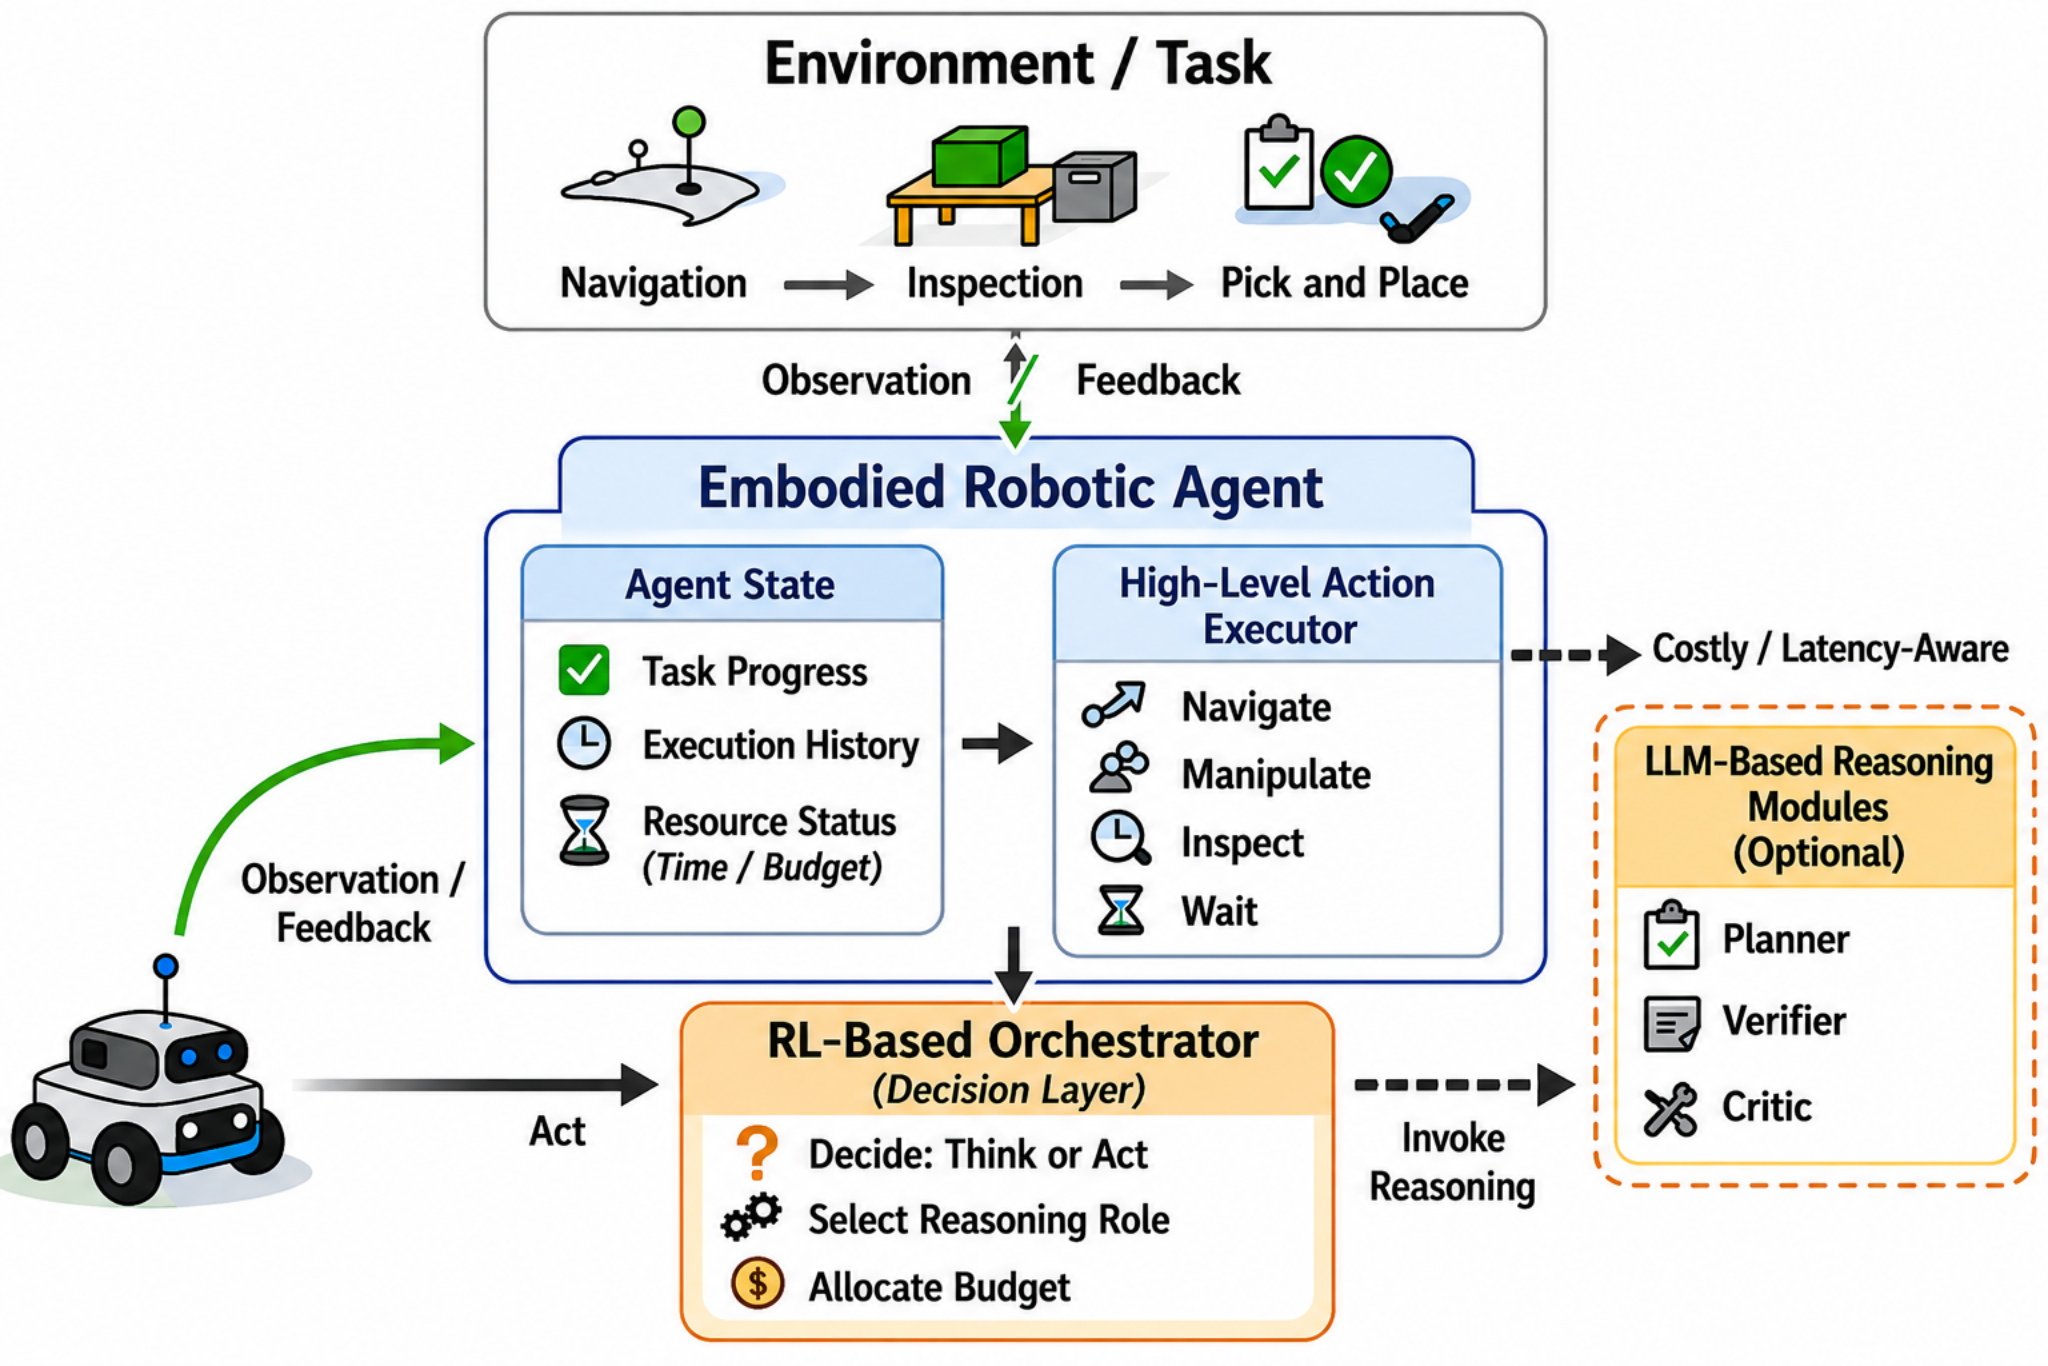
\includegraphics[width=\linewidth,keepaspectratio]{RL.png}
    \end{column}
    \begin{column}{0.36\textwidth}
      \centering
      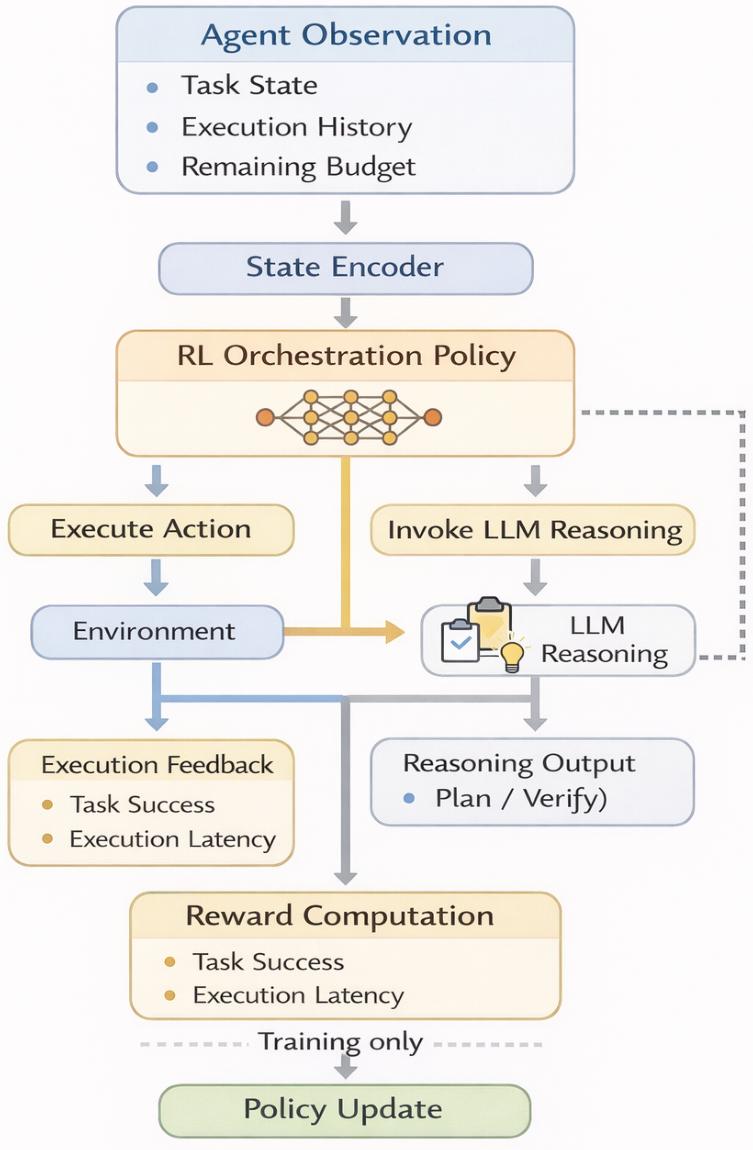
\includegraphics[height=0.80\textheight,keepaspectratio]{figure 1.png}
    \end{column}
  \end{columns}
\end{frame}
% Experiment section: three frames, approximately one minute per frame.
% The image is a conceptual illustration, not a screenshot from AI2-THOR.
% Sources: zzffzz2003/rarrl-reproduction, branch nov13-ppt-materials,
% 11月13号PPT资料/01_程序/code3d_seg/segments.py and segment_env.py;
% 11月13号PPT资料/02_数据/抽象环境/calibration3d.json.
\begin{frame}{Kitchen task and reasoning budget}
  \textbf{AI2-THOR kitchen:} each episode combines 3--4 recipes.\\[2pt]
  The controller chooses a reasoning level before each subtask.

  \medskip
  \begin{columns}[c,onlytextwidth]
    \begin{column}{0.65\textwidth}
      \centering
      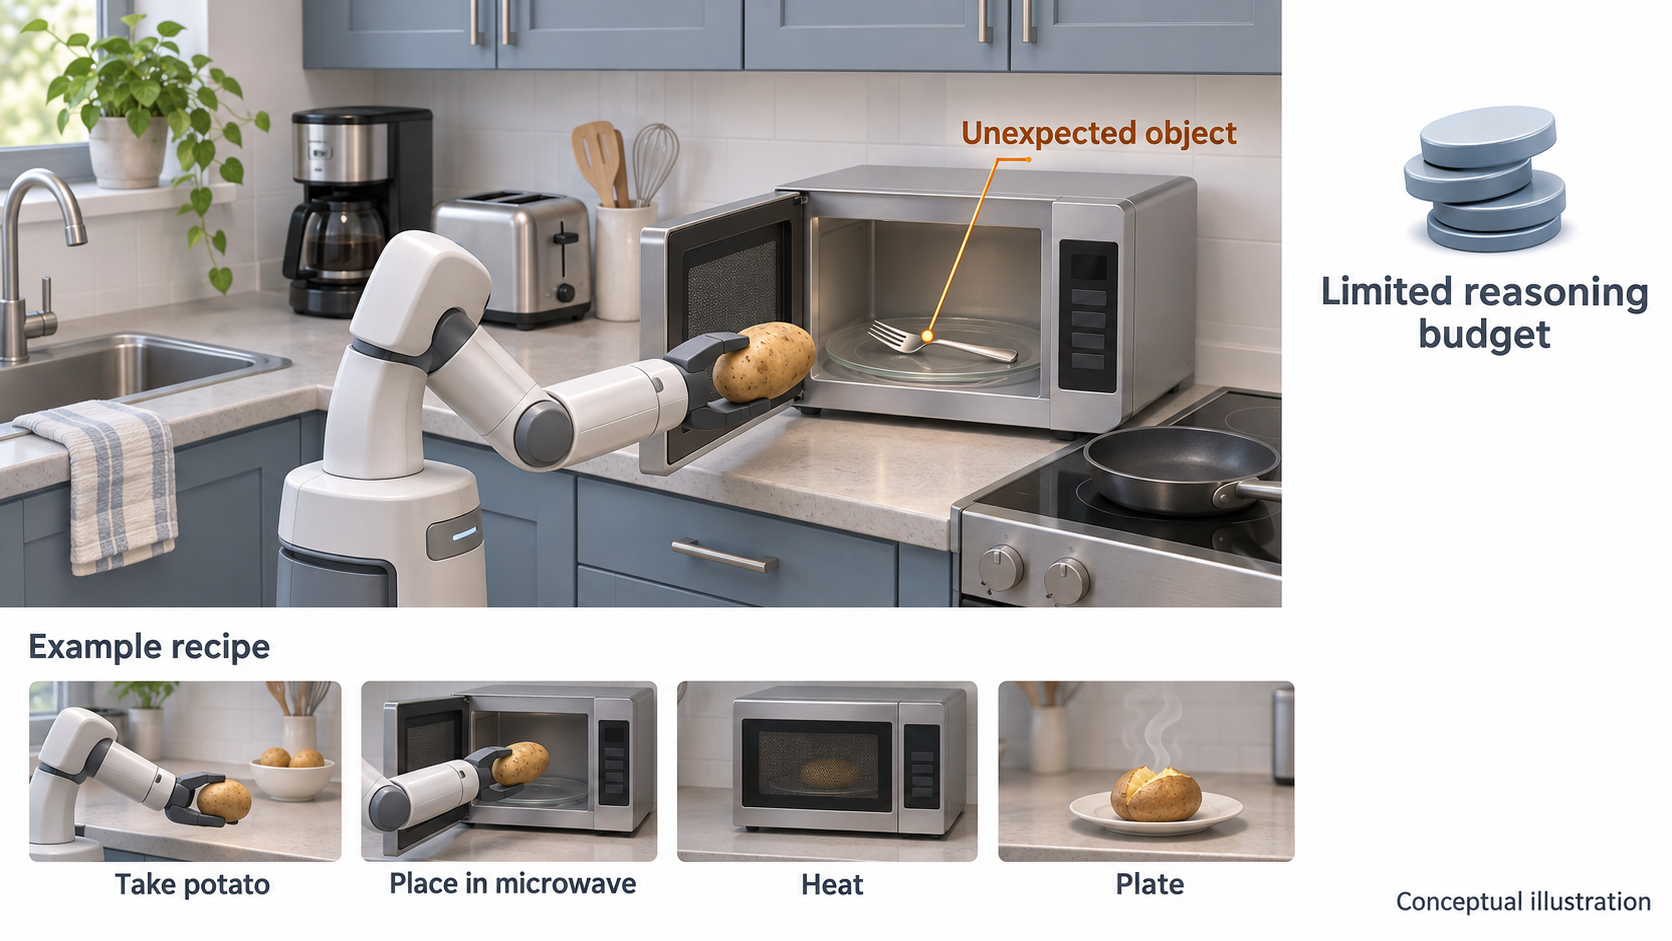
\includegraphics[width=\linewidth]{illustration figure.png}
    \end{column}
    \begin{column}{0.32\textwidth}
      \textbf{Routine steps}\\[3pt]
      Fixed scripts handle the normal recipe.

      \medskip
      \textbf{Unexpected conditions}\\[3pt]
      LLM planning can address hazards, but adds cost and may introduce errors.
    \end{column}
  \end{columns}

  \medskip
  \textbf{Limited budget:} approximately 1,400--4,100 tokens per episode.
  \note{About 60 seconds. Our robot prepares several dishes in a simulated kitchen.
  Each recipe is divided into subtasks, such as taking a potato, placing it in the
  microwave, heating it, and putting it on a plate. A fixed script handles the
  routine sequence. If a fork is already inside the microwave, following the
  script through heating triggers a rule-defined safety violation. Calling Luna
  may resolve the problem, but consumes tokens and can introduce planning errors.
  The budget cannot cover reasoning at every subtask. We also add decoys, such as
  an apple in the microwave, so an extra object does not always imply a severe
  hazard. The picture is a conceptual illustration.}
\end{frame}

% Sources: scheduler2/sched_features.py, ppo.py, run.py and breakfast3d.py;
% code3d_seg/obs3d.py, segment_env.py and eval3d.py in the same experiment folder.
\begin{frame}{Learning the Reasoning Controller}
  \begin{columns}[c,onlytextwidth]
    \begin{column}{0.29\textwidth}
      \textbf{Inputs}\par\smallskip
      Current subtask cues\par\smallskip
      Budget and progress\par\smallskip
      Recent execution results
    \end{column}
    \begin{column}{0.24\textwidth}
      \centering
      {\large\color{structure.fg}\textbf{Reasoning\\Controller}}\par
      \smallskip
      Small policy network\par
      trained with PPO
    \end{column}
    \begin{column}{0.43\textwidth}
      \textbf{One choice per subtask attempt}\par\smallskip
      \textbf{0}\quad Fixed script\par\smallskip
      \textbf{1}\quad Luna low effort\\
      \hspace*{1.6em}Compact context\par\smallskip
      \textbf{2}\quad Luna high effort\\
      \hspace*{1.6em}Full context
    \end{column}
  \end{columns}

  \bigskip
  \textbf{Reward:} task completion, minus failure and computation costs.

  \medskip
  \textbf{Training:} PPO in a simulator calibrated from 3D measurements.\\[3pt]
  \textbf{Evaluation:} freeze the controller and run actual LLM calls in 3D.

  \medskip
  \textcolor{codeMuted}{Luna's parameters remain fixed throughout.}
  \note{About 60 seconds. We train a small Reasoning Controller. It receives a
  42-dimensional observation containing subtask cues, such as whether an appliance
  contains another object or a vessel is dirty, together with budget, progress,
  and recent execution results. The controller chooses a fixed script, Luna with
  low reasoning effort and compact context, or Luna with high reasoning effort
  and full context. Level 2 is one high-effort planning call, not a separate
  planner-verifier sequence. We first measure outcomes and token costs in 3D,
  calibrate a stochastic simulator, and train PPO there. Reward favors completing
  the whole task while penalizing failures and execution and reasoning costs.
  We then freeze the controller and evaluate actual execution in 3D. Luna is
  never fine-tuned.}
\end{frame}

% Results: 11月13号PPT资料/04_已有总结/第四步_3D对比_去掉双蛋任务.md.
% Task filtering: 60 candidate tasks, 24 removed by recipe composition because
% fried_egg and egg_to_bowl compete for the single egg, leaving 36 paired tasks.
% Calibration overlap: calib_0.jsonl and calib_1.jsonl include test kitchens
% 3, 6, 10 and 13. These kitchens are held out from PPO training trajectories,
% but not all are held out from simulator calibration.
\begin{frame}{3D evaluation}
  \textbf{36 tasks.} The same task configurations for all three policies.

  \bigskip
  \begin{center}
    \renewcommand{\arraystretch}{1.45}
    \setlength{\tabcolsep}{10pt}
    \begin{tabular}{@{}lrr@{}}
      \hline
      \textbf{Policy} & \textbf{Task success} & \textbf{Tokens / episode} \\
      \hline
      Fixed scripts only & 28\% & 0 \\
      Tuned feature rule & 67\% & 1,547 \\
      \textbf{PPO Reasoning Controller} & \textbf{72\%} & \textbf{1,166} \\
      \hline
    \end{tabular}
  \end{center}

  \medskip
  \begin{center}
    {\Large\color{structure.fg}\textbf{25\% fewer tokens}}\\[4pt]
    than the tuned feature rule
  \end{center}

  \medskip
  {\small
  One PPO seed in 3D. Success-rate difference vs.\ tuned rule: not statistically significant.\par\smallskip
  \textcolor{codeMuted}{Test kitchens are held out from PPO training, with partial overlap in calibration data.}}
  \note{About 60 seconds. On 36 paired test tasks, fixed scripts succeed in 28
  percent of episodes. The tuned feature rule reaches 67 percent, and our frozen
  PPO Reasoning Controller reaches 72 percent. That success-rate difference is
  not statistically significant, so the main observation is the lower inference
  cost: 1,166 tokens per episode versus 1,547, a reduction of about 25 percent.
  The experiment provides preliminary evidence that learned reasoning control
  can reduce token use. A larger evaluation with multiple PPO seeds is needed
  to establish a consistent success-rate improvement.
  For questions: exact success counts are 10/36, 24/36, and 26/36. The reported
  paired bootstrap 95 percent interval for PPO minus the tuned rule is -8.3 to
  +19.4 percentage points. The controller is medium-s100, selected by validation
  return. Rules are also tuned on validation tasks. Test kitchens do not appear
  in PPO training trajectories, but some appear in the 3D calibration data.
  Strict calibration holdout is future work.}
\end{frame}
\end{document}
